\section{Autoformer Model}
\label{sec:Autoformer}

This work applies the Autoformer framework to optimize and fine-tune pre-trained models on custom datasets. The Autoformer framework, downloaded from Hugging Face, is designed to capture the temporal dependencies of time-series data through advanced temporal encoding and self-attention mechanisms. We adjusted the model's hyperparameters to suit the dataset characteristics, achieving improved forecasting performance.

\subsection{Autoformer Hyperparameters and Input Parameters}
\label{subsec:AutoformerParams}

\subsubsection{Hyperparameters}
\begin{itemize}
	\item \textbf{prediction\_length}: Defines the number of time steps the model predicts into the future.
	\item \textbf{context\_length}: Specifies the length of the historical window used as input to provide context for predictions.
	\item \textbf{label\_length}: Indicates the length of the decoder's input sequence during training, usually equal to the prediction length.
	\item \textbf{moving\_average}: Sets the size of the moving average window used to smooth input data and reduce noise.
	\item \textbf{lags\_sequence}: A sequence of lag indices (e.g., \([4, 7, 11]\)) used as additional features by including values from previous time steps.
	\item \textbf{target\_distribution}: Specifies the type of target distribution (e.g., \textit{normal} for Gaussian distribution) used to model prediction uncertainty.
\end{itemize}

\subsubsection{Input Parameters}
\begin{itemize}
	\item \textbf{past\_values}: Historical time series values with a shape of \((\textit{batch\_size}, \textit{context\_length})\), providing information about historical trends.
	\item \textbf{past\_time\_features}: Temporal features corresponding to historical values with a shape of \((\textit{batch\_size}, \textit{context\_length}, \textit{num\_time\_features})\).
	\item \textbf{past\_observed\_mask}: A mask matrix of shape \((\textit{batch\_size}, \textit{context\_length})\), indicating valid data points in historical values.
	\item \textbf{future\_time\_features}: Temporal features for future time steps with a shape of \((\textit{batch\_size}, \textit{prediction\_length}, \textit{num\_time\_features})\).
	\item \textbf{future\_values}: Ground truth future time series values of shape \((\textit{batch\_size}, \textit{prediction\_length})\) used as targets during training.
\end{itemize}

\section{Experimental Process}
\label{sec:Experiment}

\subsection{Parameter Selection}
\label{subsec:ParameterSelection}
Initially, the dataset of Component 3 was used as the validation set to optimize hyperparameters. The final parameters selected for training were as follows:
\begin{itemize}
	\item \textbf{context\_length}: 9
	\item \textbf{prediction\_length}: 1
	\item \textbf{lags\_sequence}: \([4, 7, 11]\)
	\item \textbf{moving\_average}: 5
	\item \textbf{num\_paraller\_samples}: 1
	\item \textbf{batch\_size}: 32
\end{itemize}

\subsection{Model Training}
\label{subsec:Training}
Component 4 was used as the training dataset. The dataset was divided such that the first 20 time steps were used to predict the 21st time step, followed by using time steps 2 to 21 to predict the 22nd time step, and so on. All values for the first 20 time steps were passed as \textit{past\_values}, and the corresponding future values were passed as \textit{future\_values}. The AdamW optimizer was used for training, and the loss values for the optimal model at various learning rates and epochs were as follows:
\begin{table}[h]
	\centering
	\begin{tabular}{|c|c|c|}
		\hline
		\textbf{Epoch} & \textbf{Learning Rate (lr)} & \textbf{Loss} \\
		\hline
		5 & $1\times10^{-4}$ & 4.284 \\
		5 & $1\times10^{-5}$ & 4.535 \\
		10 & $1\times10^{-4}$ & 3.941 \\
		10 & $1\times10^{-5}$ & 4.053 \\
		20 & $1\times10^{-5}$ & 2.762 \\
		20 & $1\times10^{-4}$ & 2.418 \\
		\hline
	\end{tabular}
	\caption{Model Loss at Different Learning Rates and Epochs}
	\label{tab:loss_table}
\end{table}

\subsection{Model Testing}
\label{subsec:Testing}
The best-trained model was tested on Component 5. Since the test set was split by date, each record's month and date were extracted as \textit{time\_features}. Predictions were made for the next 8 and 22 time steps, respectively:
\begin{itemize}
	\item \textbf{8 Time Steps:}
		\begin{itemize}
		\item Mean Squared Error (MSE): 1.0037
		\item Mean Absolute Error (MAE): 0.8762
	\end{itemize}
	\begin{figure}[h!]
		\centering
		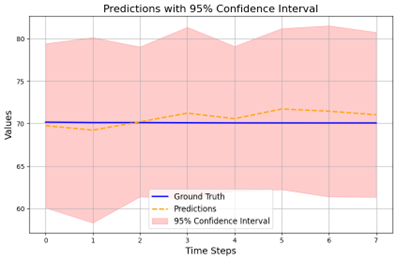
\includegraphics[width=0.8\linewidth]{figures/8times_before}
		\caption{Results for 8 Time Steps}
		\label{fig:8times_before}
	\end{figure}

\end{itemize}


\begin{itemize}
	\item \textbf{22 Time Steps:}
	\begin{figure}[h!]
		\centering
		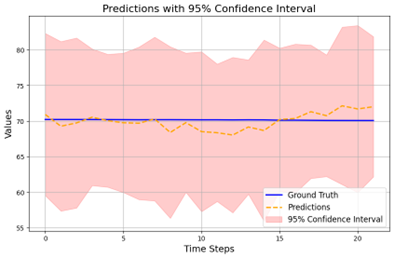
\includegraphics[width=0.8\linewidth]{figures/22times_before}
		\caption{Results for 22 Time Steps}
		\label{fig:22times_before}
	\end{figure}

\end{itemize}
	\begin{itemize}
	\item Mean Squared Error (MSE): 1.4571
	\item Mean Absolute Error (MAE): 0.9907
\end{itemize}

Despite close alignment with the ground truth, the predicted values showed higher fluctuations compared to the nearly steady ground truth. To address this, we applied a moving average:

\begin{equation}
	y_t^{\text{smooth}} = \alpha y_t + (1-\alpha)y_{t-1}^{\text{smooth}}
\end{equation}
where $\alpha \in (0, 1)$ controls the degree of smoothing. The smaller the value of $\alpha$, the smoother the predictions.

with $\alpha=0.01$ for smoothing the predictions.for smoothing the predictions. After smoothing, the results for the next 22 time steps on Component 5 were:

\begin{itemize}
	\item \textbf{22 Time Steps After Smoothing:}
	\item Mean Squared Error (MSE): 0.0989
	\item Mean Absolute Error (MAE):0.0109
\end{itemize}
	\begin{figure}[h!]
	\centering
	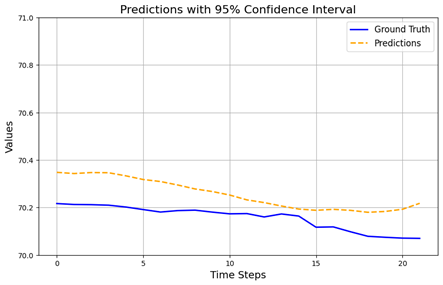
\includegraphics[width=0.8\linewidth]{figures/22no5}
	\caption{Results for 22 Time Steps After Smoothing}
	\label{fig:22no5}
\end{figure}
It can be observed that after applying the smoothing process, the model achieves excellent prediction performance on the Component 5 dataset.
\subsection{Performance on Other Datasets}
\label{subsec:Performance}
The model was further tested on Components  6, 7, and 8 for the next 22 time steps. Results are summarized below:

\begin{itemize}
	\item \textbf{22 Time Steps on No.6 After Smoothing:}
	\item Mean Squared Error (MSE): 0.2102
	\item Mean Absolute Error (MAE):0.0446
\end{itemize}
\begin{figure}[h!]
	\centering
	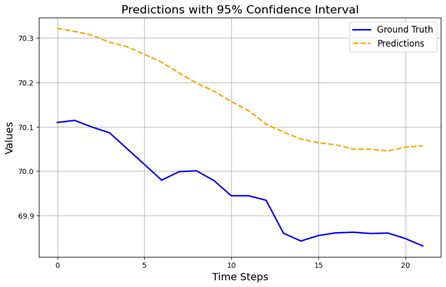
\includegraphics[width=0.8\linewidth]{figures/22no6}
	\caption{Results for 22 Time Steps  on No.6 After Smoothing}
	\label{fig:22no6}
\end{figure}
\begin{itemize}
	\item \textbf{22 Time Steps on No.7 After Smoothing:}
	\item Mean Squared Error (MSE):0.2927
	\item Mean Absolute Error (MAE): 0.1008
\end{itemize}
\begin{figure}[h!]
	\centering
	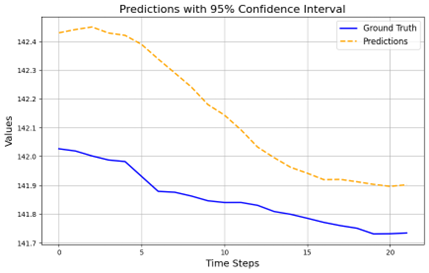
\includegraphics[width=0.8\linewidth]{figures/22no7}
	\caption{Results for 22 Time Steps  on No.7 After Smoothing}
	\label{fig:22no7}
\end{figure}
\begin{itemize}
	\item \textbf{22 Time Steps on No.8 After Smoothing:}
	\item Mean Squared Error (MSE):0.6869
	\item Mean Absolute Error (MAE):0.5087
\end{itemize}
\begin{figure}[h!]
	\centering
	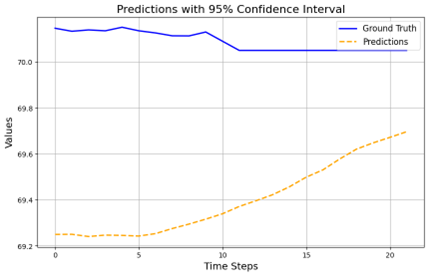
\includegraphics[width=0.8\linewidth]{figures/22no8}
	\caption{Results for 22 Time Steps  on No.8 After Smoothing}
	\label{fig:22no8}
\end{figure}
The results demonstrate strong model performance on datasets with declining trends. However, for datasets with flat or increasing trends, prediction accuracy was comparatively